\section{Lecture 5: Superscalar Architecture (SSA)}
Computer designed to improve computation on scalars instructions.
A scalar is a variable that can hold only one atomic value at a time, e.g., an integer or a real.
A scalar architecture processes one data item at a time -- the computers we discussed up till now.
Examples of non-scalar variables:
\begin{itemize}
\item Arrays -- Vector Processor
\item Matrices -- Graphics Processing Unit (GPU)
\item Records
\end{itemize}

In a superscalar architecture (SSA), several scalar instructions can be initiated simulaneously and executed independently.

\subsection{Instruction-level parallelism}
Most operations are on scalar quantities, speed up these operations will lead to large performance improvement.

\subsubsection{Superpipelining}
Superpipelining exploits the fact that many pipeline stages perform tasks that require less than half a clock cycle. Thus, a doubled internal clock speed allows the performance of two tasks in one external clock cycle.

We divide pipelining stages into several sub-stages, and hence increase the number of instructions which are handled by the pipeline at the same time. But note that although several instructions are executing concurrently, only one instruction is in its execution stage at any one time.

\todo{A picture would be nice here} \\

\begin{enumerate}
\item For example by diving each stage into two sub stages, we will be able (in the ideal situation) to perform each stage at twice the speed.
\item No duplication of hardware is needed. 
\item Not all stages can be divided into (equal length) sub stages.
\item Hazards more difficult to resolve.
\item More complex hardware.
\item Interrupt handling and testing will be more complicated.
\end{enumerate}
  
\subsubsection{Difference between Superpipelined and Superscalar Designs}
The difference is that Superpipeline can perform several instructions in one clock cycle, whereas Superscalar performs several instructions in parallel

\begin{figure}[H]
  \centering
  \scalebox{0.342}{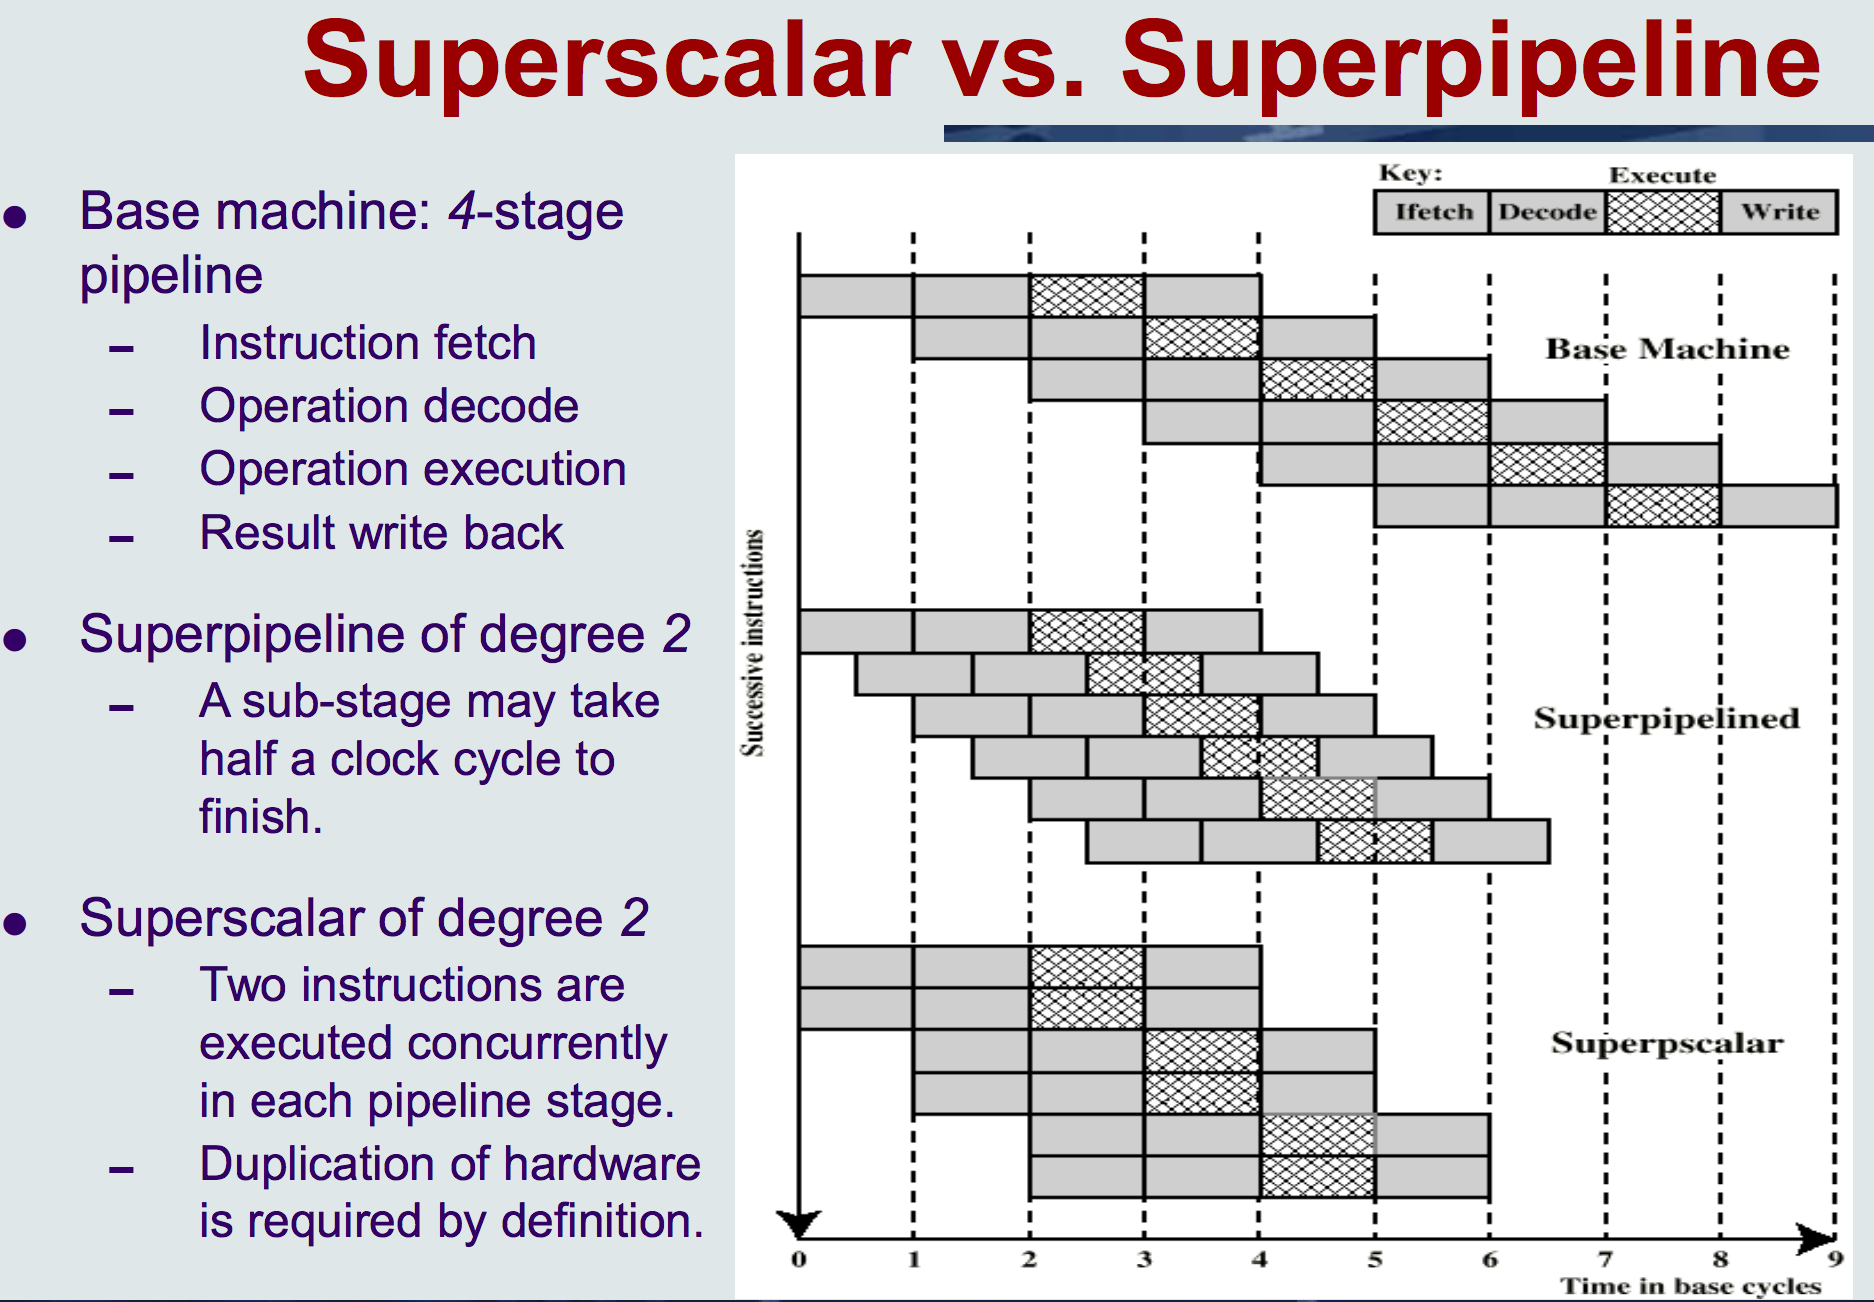
\includegraphics{img/superscalar-vs-superpipeline.png}}
  \caption{Difference between a Superscalar and a Superpipeline architecture}
  \label{fig:superscalar-vs-superpipeline}
\end{figure}


\subsubsection{Superscalar Superpipeline Design}

\begin{figure}[H]
  \centering
  \scalebox{0.342}{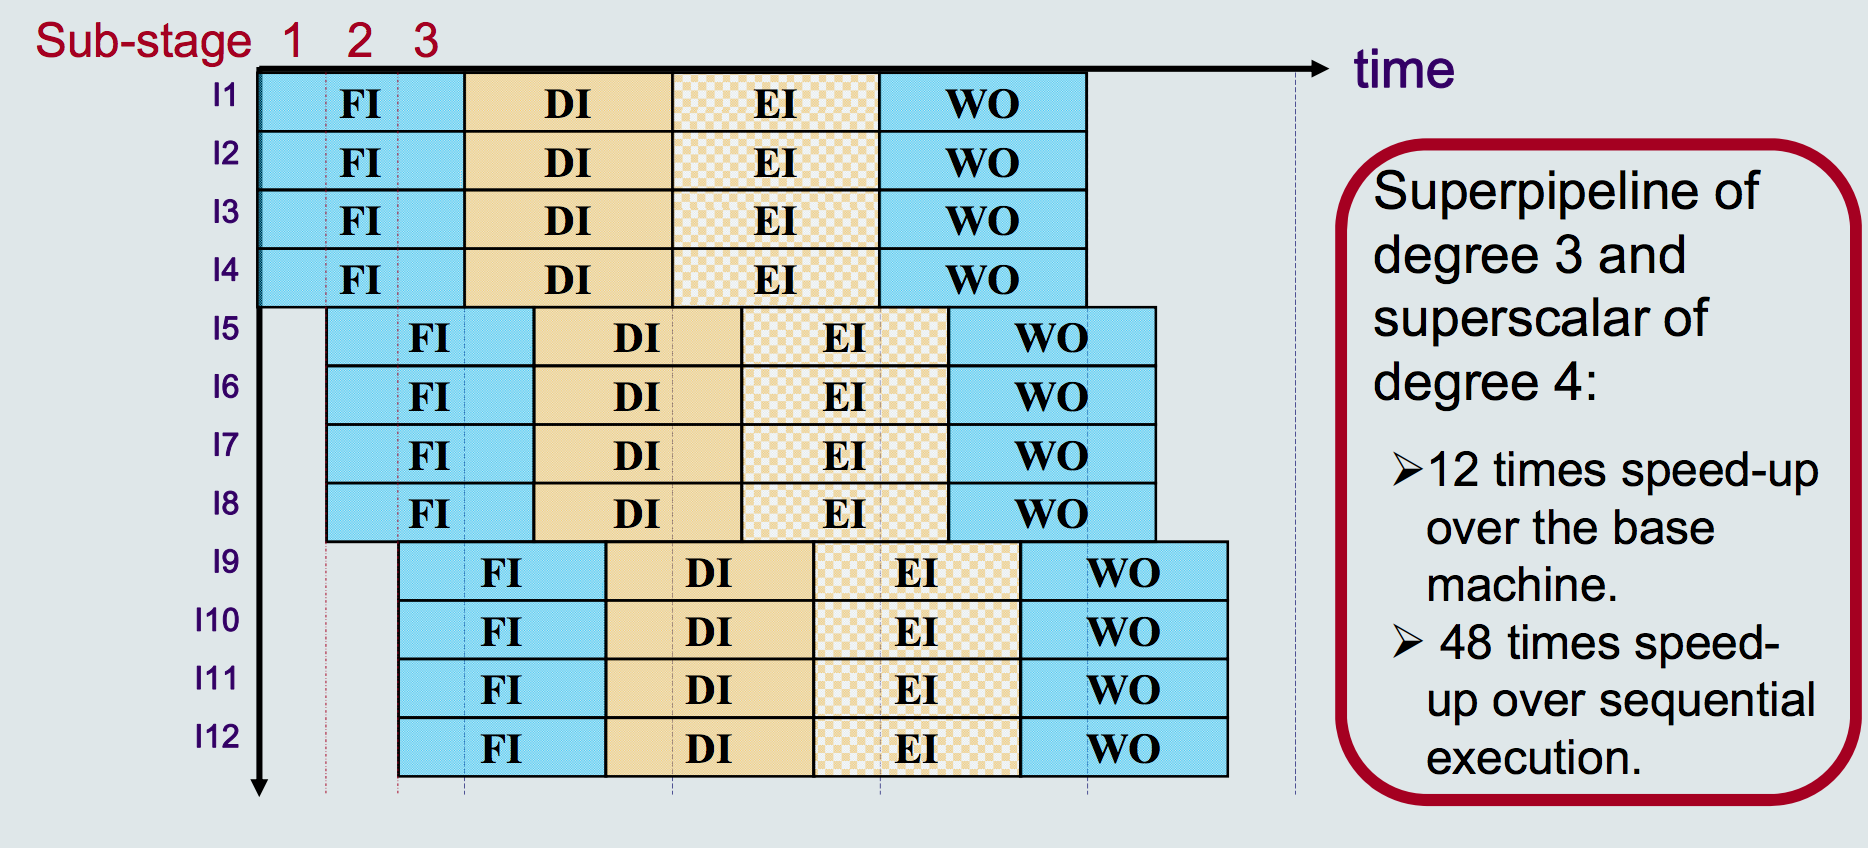
\includegraphics{img/superscalar-superpipeline.png}}
  \caption{Superscalar Superpipeline architecture}
  \label{fig:superscalar-superpipeline}
\end{figure}

The new trend is to combined the two ideas. In Figure \ref{fig:superscalar-superpipeline} it says that this would give us a 48 times speedup, this is not the case though because of data dependencies.

\subsection{Dependency issues}
The superscalar approach depends on the ability to execute multiple instructions in parallel. The term instruction-level parallelism refers to the degree to which, on average, the instructions of a program can be executed in parallel. A combination of compiler-based optimization and hardware techniques can be used to maximize instruction-level parallelism.

The main problems are:
\begin{itemize}
\item Resource conflicts.
\item Control (procedural) dependency.
\item Data dependencies.
\item True data dependency.
\item Output dependency.
\item Anti Dependency.
\end{itemize}
  
These are very similar to the cases in normal pipelining (data hazards). But the consequences are more severe here because the parallelism are greater and thus larger amount of performance will be lost.

\subsubsection{Resource Conflicts}
Several instructions compete for the same hardware resource at the same time.
\begin{itemize}
\item For instance, two aritmethic instructions need the same floating-point unit for execution.
\item similar to structural hazards in pipeline.
\end{itemize}

They can be solved \underline{partly} by introducing several hardware units for the same functions.
\begin{itemize}
\item e.g. have two floating point units.
\item the hardware units can also be pipelined to support several operations at the same time.
\item however, memory units \textbf{can't be duplicated}.
\end{itemize}
  
\subsubsection{Procedural Dependency}
The instructions following a branch (taken or not taken) have a procedural dependency on the branch and cannot be executed until the branch is executed.

As with regular pipelining, this type of procedural dependency also affects a scalar pipeline. The consequence for a superscalar pipeline is more severe, because a greater magnitude of opportunity is lost with each delay.

If variable-length instructions are used, then another sort of procedural dependency arises. Because the length of any particular instruction is not known, it must be at least partially decoded before the following instruction can be fetched. This prevents the simultaneous fetching required in a superscalar pipeline. This is one of the reasons that superscalar techniques are more readily applicable to a RISC or RISC-like architecture, with its fixed instruction length.

\subsubsection{Data Conflicts}
These are caused by dependencies between instructions in the program. They are similar to data hazards in regular pipelining, but they cause more problems due to that we much more data dependencies because of parallel execution of many instructions.

To address the problem and to increase the degree of parallel execution, SSA provides a great liberty in the order in which instructions are issued and executed. Therefore, data dependencies have to be considered and dealt with much more carefully.
\subsubsection{Window of execution}
Because of data dependencies, only some instructions are able to execute in parallel. The processor has to select from a sufficiently large instruction set. \textbf{Window of execution} is then the set of instructions that is considered to be able to execute in parallel at a certain moment.

The number of instructions in the window should be as large as possible, however it is limited by: \\
\begin{itemize}
\item Capacity to fetch instructions at a high rate.
\item The problem of branches.
\item The cost of hardware needed to analyze data dependencies (we don't really care about cost, we want to build cool stuff)
\end{itemize}

The window of execution can be extended over basic block borders by branch prediction (\textbf{speculative execution}).

\textbf{Speculative execution} works like this:
\begin{enumerate}
\item Instructions of the predicted path are entered into the window of execution.
\item If the prediction turns out to be correct, we were able to do some of them in advance (which is superduper), and the changes will become permanent and visible (they will \textbf{commit})
\item If not, all changes will undone, and the result will be ignored.
\end{enumerate}

\subsubsection{Data Dependencies}
All instructions in the window of execution may begin execution, subject to data dependence and resource constraints.
\begin{itemize}
\item True data dependency
\item Output dependency
\item Anti dependency
\end{itemize}

\subsubsection{True Data Dependency}
True data dependencies exist when the output of one instruction is required as an input to a subsequent instruction:
\begin{lstlisting}[frame=single]  % Start your code-block
  . . .
  MUL R4,R3,R1 (R4 := R3 * R1)
  . . .
  ADD R2,R4,R5 (R2 := R4 + R5)
\end{lstlisting}
In this example we can fetch and decode the second instruction in parallel, but we have to wait to perform it because its dependant on registers from the first instruction.

They are intrinsic features of a program, and cannot be eliminated by compiler or hardware techniques. The hardware have to detect them, and solve them. The easiest way to do this in this example, is just to stall the first instruction until we can perform the second.

This type of depency is very common, and by increasing the window size we can reduce the impact of them. \\

\subsubsection{Anti Dependency}
Also known as write after read, occurs when an instruction requires a value that is later updated. In the code block below, instruction 2 is anti-dependant on instruction 3. The ordering of the instructions cannot be changed, nor can the instructions be executed in parallel. 
\begin{lstlisting}[frame=single]  % Start your code-block
  . . .
  1. B = 3
  2. A = B + 1
  3. B = 7
\end{lstlisting}

Anti-dependcies are naming dependencies, renaming of variables could remove the dependency, as seen in the code below. \\

\begin{lstlisting}[frame=single]  % Start your code-block
  . . .
  1. B = 3
  N. B2 = B
  2. A = B2 + 1
  3. B = 7
\end{lstlisting}

\subsubsection{Output Dependency}
An output dependency, also known as write-after-write (WAW), occurs when the ordering of instructions will affect the final output value of a variable. In the example below, there is an output dependency between instructions 3 and 1 — changing the ordering of instructions in this example will change the final value of A, thus these instructions cannot be executed in parallel.

\begin{lstlisting}[frame=single]  % Start your code-block
  . . .
  1. B = 3
  2. A = B + 1
  3. B = 7
\end{lstlisting}

As with anti-dependencies, output dependencies are name dependencies. That is, they may be removed through renaming of variables, as in the below modification of the above example:

\begin{lstlisting}[frame=single]  % Start your code-block
  . . .
  1. B2 = 3
  2. A = B2 + 1
  3. B = 7
\end{lstlisting}

\subsection{Parallel instruction execution}
\subsubsection{Instruction vs Machine Parallelism}
\subsubsection{Division and Decoupling}
\subsubsection{SSA instruction Execution Policies}
\subsubsection{In-Order with In-Order Completion}
This seems important to understand
\subsubsection{In-Order issue with Out-of-Order Completion}
This seems important to understand
